\documentclass{beamer}
\usetheme{default}
\useoutertheme{infolines}
\usepackage{graphicx}
\usepackage{hyperref}

% logo
\logo{
\includegraphics[height=0.1\textwidth]{./images/rock.png}}

\title{Rock Your Page}
\subtitle{A Chrome Extension Makes Your Webpage More Controlled}
\author{\and{WANG Yue}\and{LUO Xuan}\and{LI Zhi}}
\institute[HKUST]{
    Department of Computer Science \\
    Hong Kong University of Science and Technology \\
}
\date{November 14, 2013}


\begin{document}
\begin{frame}[plain]
    \titlepage
\end{frame}

%%%%%%%%%%%%%%%%%%%%%%%% For Luoxuan: Product Manager %%%%%%%%%%%%%%%%%%%%%%%%
% Motivation
\begin{frame}{Rock Your Page: Motivation}
How do we get the final product idea?
\bigskip

\begin{columns}[t]
    \begin{column}{0.33\textwidth}
        Start Point: 
        \begin{itemize}
            \item Screen of Laptop $\Longrightarrow$ smaller
            \item Font of web pages sometimes not suitable
        \end{itemize}

        Change size of web pages automatically
    \end{column}
    \begin{column}{0.33\textwidth}
        One Step Further
        \begin{itemize}
            \item Given a webpage, what can we do about it?
        \end{itemize}

        map several webpages into one, for easily browsing
    \end{column}
    \begin{column}{0.33\textwidth}
        Final Idea:
        \begin{itemize}
            \item two tools
            \item one small game
        \end{itemize}
    \end{column}
\end{columns}
\end{frame}
% Overview Features
% Three components
\begin{frame}{Rock Your Page: Features Overview}
Three Components:
\begin{itemize}
    \item Page Sizer: adjust size of contents in web pages based on distance between your face and screen automatically.
    \item Page Rotater: map your 2D web page into 3D scene, multiple pages projection is also supported.
    \item Page Rocker: a small game which let your web page dance with music.
\end{itemize}
\begin{center}
    \begin{figure}
        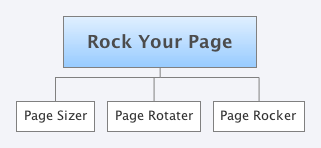
\includegraphics[width=0.4\textwidth]{./images/Rock_Your_Page.png}
        \caption{Overview of Components}
\end{figure}
\end{center}
\end{frame}

\begin{frame}{Rock Your Page: Prototype}
    \begin{center}
        \begin{figure}
            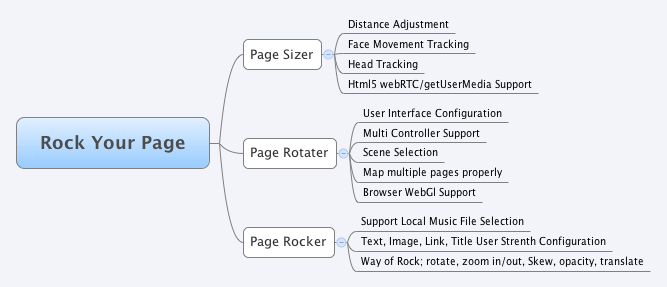
\includegraphics[width=0.8\textwidth]{./images/prototype.png}
            \caption{Prototype Design}
        \end{figure}
    \end{center}
\end{frame}

%%%%%%%%%%%%%%%%%%%%%%% For Wangyue: technical details %%%%%%%%%%%%%%%%%%%%%%%%
%% Functions
%% Technical Details
% chrome extension
\begin{frame}{Technical Overview: Chrome Extension Development}
    \begin{figure}
        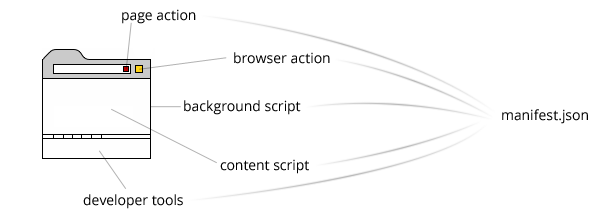
\includegraphics[width=0.8\textwidth]{./images/architecture.png}
        \caption{Architecture of Chrome Extension}
    \end{figure}
\end{frame}

\begin{frame}{Technical Details: Page Sizer}
\begin{center}
    \begin{figure}
        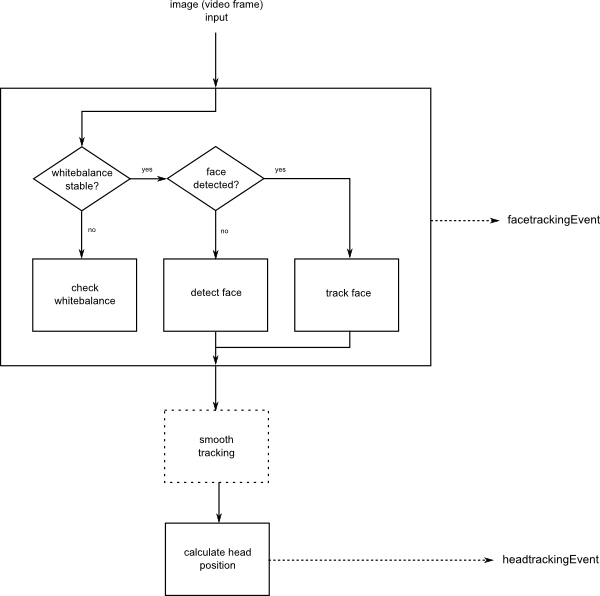
\includegraphics[width=0.6\textwidth]{./images/face_detectin.png}
        \caption{Face Detection in JavaScript}
    \end{figure}
\end{center}
\end{frame}

\begin{frame}{Technical Details: Page Sizer}
\begin{center}
    \begin{figure}
        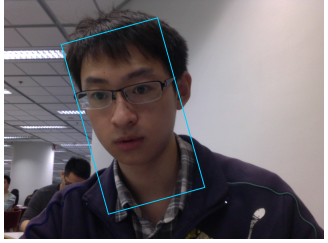
\includegraphics[width=0.25\textwidth]{./images/face_detection_realtime.png}
        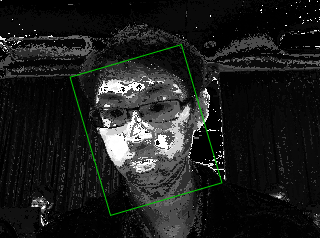
\includegraphics[width=0.25\textwidth]{./images/face_detection_possibility.png}
        \caption{Realtime Face Detection Using Web Camera(\emph{libccv})}
    \end{figure}
\end{center}
Which element in web page shouled be sized?
\begin{itemize}
    \item p,a,h1,h2,h3,h4,h5,h6,code,span,img,pre 
\end{itemize}
How should we detemine the zoom amp?
\begin{equation}
    zoom\_value = (face\_init\_width / video\_init\_width) / (face\_width / video\_width)
\end{equation}
\end{frame}

% Page Rotater
\begin{frame}{Technical Details: Page Rotater}
One single web page mapped into 3D world.
\begin{center}
    \begin{figure}
        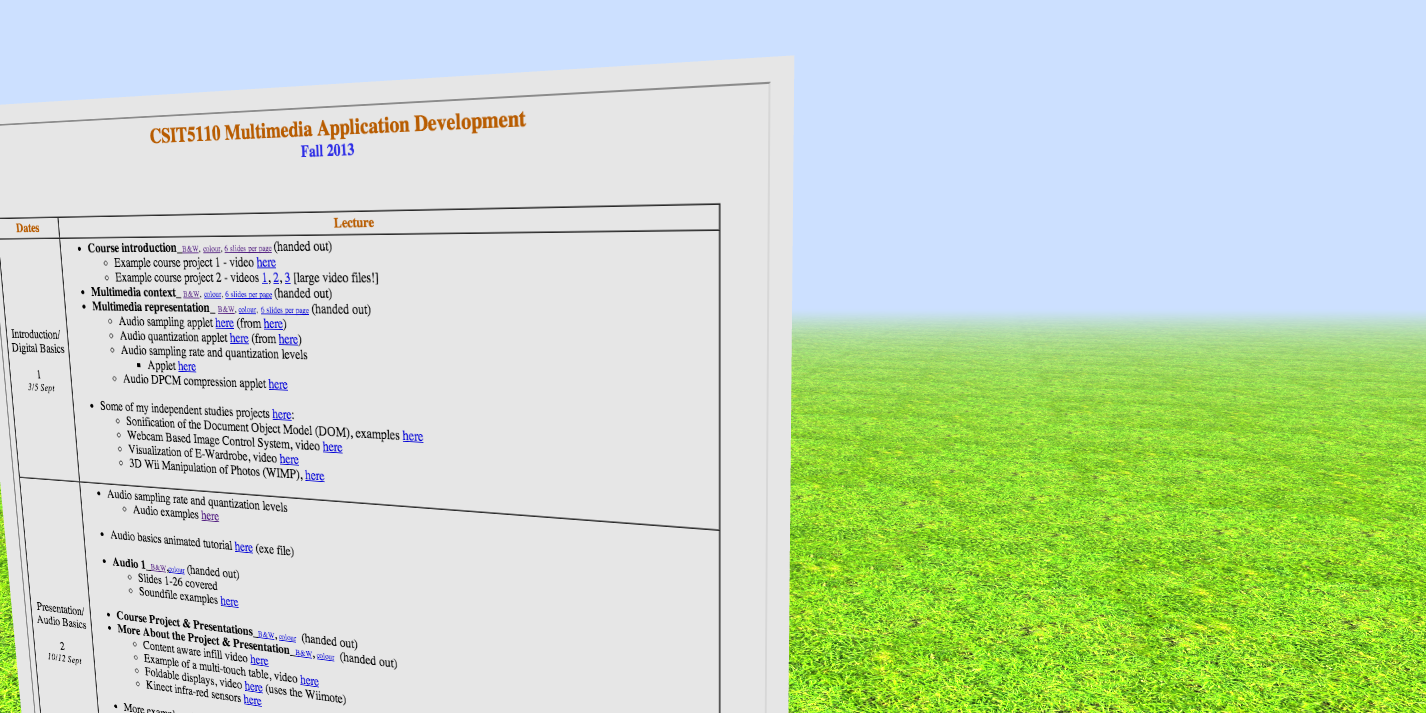
\includegraphics[width=0.8\textwidth]{./images/3d_webpage.png}
        \caption{One single Webpage Mapped to Three-Dimension Scene}
    \end{figure}
\end{center}
\begin{center}
\end{center}
\end{frame}

% multiple web pages
\begin{frame}{Technical Details: Page Rotater}
Map one or several pages into 3D world.
\begin{center}
    \begin{figure}
        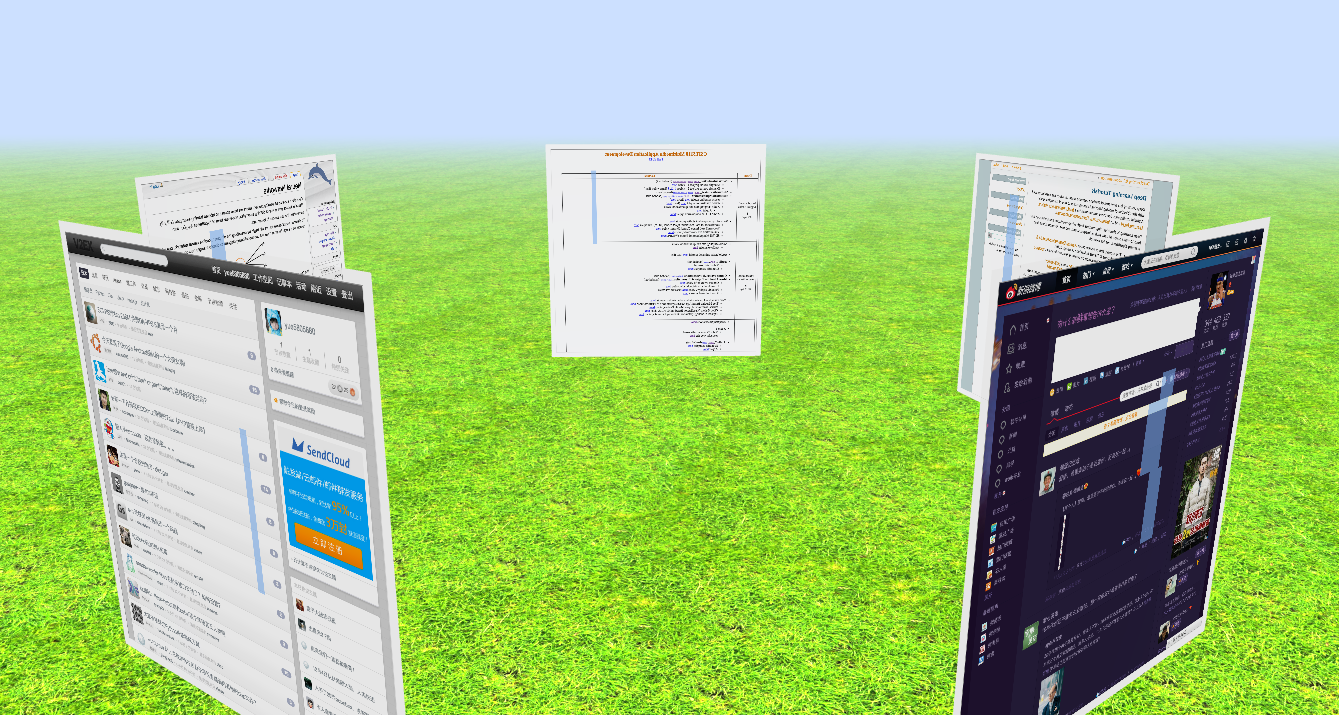
\includegraphics[width=0.8\textwidth]{./images/multi-3d-webpages.png}
        \caption{One single Webpage Mapped to Three-Dimension Scene}
    \end{figure}
\end{center}
\begin{center}
\end{center}
\end{frame}

\begin{frame}{Technical Details: Page Rotater}
How we could combine the current webpage with a 3-D Scene.
\begin{center}
    \begin{figure}
        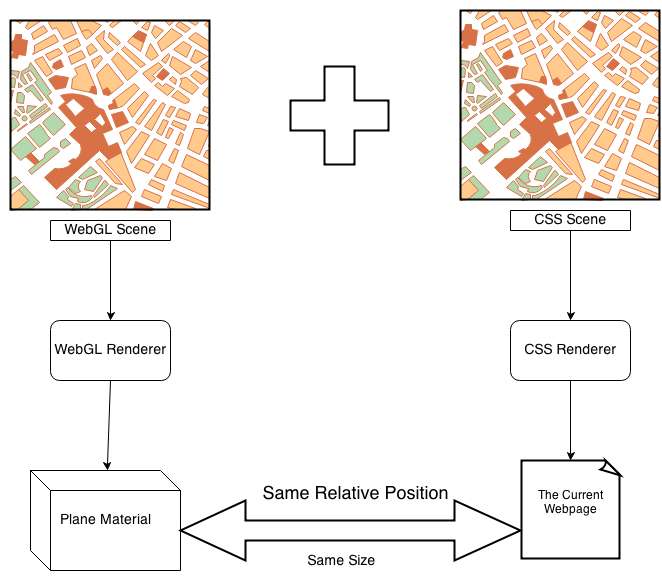
\includegraphics[width=0.5\textwidth]{./images/css3d.png}
        \caption{Map a webpage to a 3D scene}
    \end{figure}
\end{center}
So even in 3D world we can interact with our pages individually without problem.
\end{frame}

\begin{frame}{Technical Details: Page Rotater}
\begin{center}
    \begin{figure}
        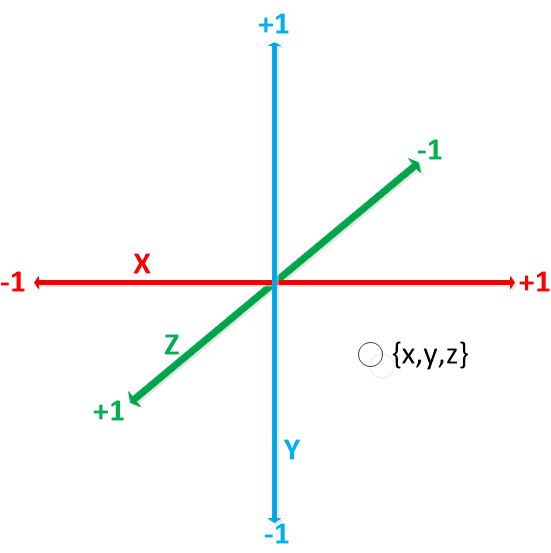
\includegraphics[width=0.5\textwidth]{./images/threejs_corodinate.png}
        \caption{The Coordinate in ThreeJS}
    \end{figure}
\end{center}
\end{frame}

\begin{frame}{Technical Details: Page Rotater}
When there n pages, how to set their position and rotation in 3D scene.
\begin{enumerate}
    \item calculate the angle for the ith webpage: $angle = \pi * 2 * i / n$
    \item The position of ith webpage: $Position_{x} = radius * sin(angle)$ and $Position_{z} = radius * cos(angle)$
    \item The rotation of ith webpage: $Vector3(0, angle, 0)$
\end{enumerate}
We provide two ways to control your page:
\begin{itemize}
    \item Orbit Controller
    \item Pointer Lock Controller
\end{itemize}
\end{frame}

% rocker technical details
\begin{frame}{Technical Details: Page Rocker}
HTML5 Web Audio Context:
\begin{center}
    \begin{figure}
        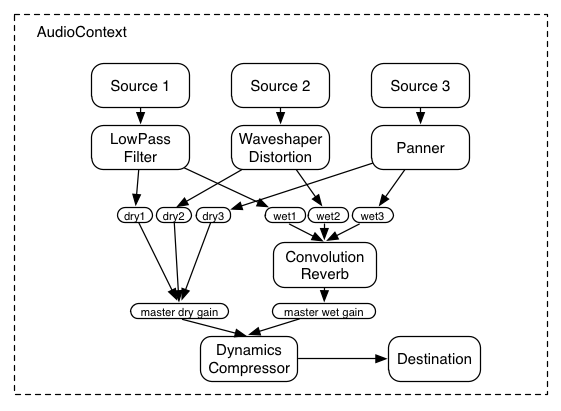
\includegraphics[width=0.7\textwidth]{./images/audiocontext.png}
        \caption{Web Audio Context}
    \end{figure}
\end{center}
\end{frame}

% different ways of rocking
\begin{frame}{Technical Details: Page Rocker}
Now Four Ways to make page dance with music:
\begin{itemize}
    \item \textbf{ZoomIn/ZoomOut}: images
    \item \textbf{Position Transition}: paragraph
    \item \textbf{Rotation}: links
    \item \textbf{Skew}: titles
\end{itemize}
\end{frame}

\begin{frame}{Technical Details: Page Rocker}
    Given An Element, how to decide their action(samples), \emph{amp} is the strength related to corresponding frequency(1 of 256):
\begin{enumerate}
    \item Fisrt we check the type of the element
    \item if \emph{images}: $Scale = -0.5 + amp $
    \item if \emph{paragraph}: $Position_{x} = -10 + 20 * amp$
    \item if \emph{link}: $Rotation = (-30 + amp * 60)$ degree
    \item if \emph{titles}: $Skew = (-30 + amp * 60)$ degree
\end{enumerate}

The general equation:
\begin{equation}
    Strengh = BaseLine + amp * Range
\end{equation}
\end{frame}

\begin{frame}{Technical Details: Page Rocker}
But we can let user decide all the rocking details by providing configuraion
\begin{center}
    \begin{figure}
        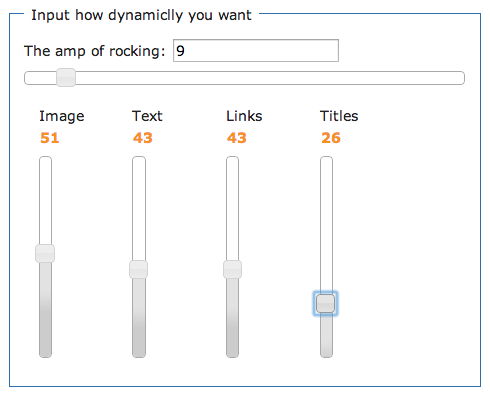
\includegraphics[width=0.5\textwidth]{./images/amp_configuration.png}
        \caption{User Configuration for Rocking}
    \end{figure}
\end{center}
Also, you can either choose one online music file or a local music file
\end{frame}

% configuraion not included
% issue
\begin{frame}{Issue: What Problems We Have Met} How to keep states for each singal webpage seperately?
\begin{itemize}
    \item write the extension states to global \emph{window} object using code injection
\end{itemize}

How to load user local file from an chrome extension dynamically?
\begin{itemize}
    \item due to security policy, not allowed in popup extension. Also using code injection, we can load user file dynamically. The request now from the webpage we are browsing.
\end{itemize}

Generally we are not allowed to modify the original web page because it's offensive to users.
\begin{itemize}
    \item Leave this problem to users, let them devide whether they trust us. But when the web site uses \emph{https} protocol, we are denied.
\end{itemize}

\end{frame}
%% Team work and other information
\begin{frame}{Development Details}
\begin{itemize}
    \item \emph{Dev Lauguage}: Javascript, HTML, CSS
    \item \emph{Project Repo}: \url{https://github.com/KeithYue/PageRocker}
    \item \emph{Team Work}:
        \begin{itemize}
            \item LUO Xuan:
                \begin{itemize}
                    \item product manager
                    \item general/specific requirements analysis, prototype design
                    \item UI design, layout and CSS implement
                \end{itemize}
            \item WANG Yue:
                \begin{itemize}
                    \item chrome extension development, set up dev env
                    \item page rotater
                \end{itemize}
            \item LI Zhi:
                \begin{itemize}
                    \item page sizer
                    \item page rocker
                \end{itemize}
        \end{itemize}
\end{itemize}
\end{frame}

% toolsets
\begin{frame}{Development Details: Toolsets}
\begin{itemize}
    \item Version Control: git version 1.8.3.4
    \item Js Library: jQuery1.9.2, ThreeJS(Revision58)
    \item Prototype Design: XMind
\end{itemize}
\end{frame}

% code frequency
\begin{frame}{Development Details}
\begin{center}
    \begin{figure}
        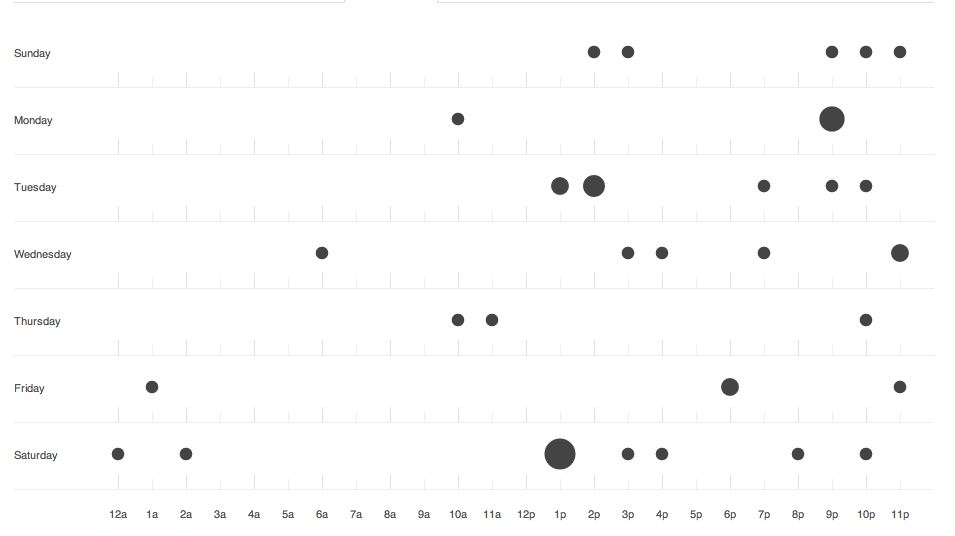
\includegraphics[width=0.9\textwidth]{./images/code_frequency.png}
        \caption{code commit frequency}
    \end{figure}
\end{center}
\end{frame}


% development details
%% development env
%% develop tools

%%%%%%%%%%%%%%%%%%%%%%% For LiZhi: Future Work %%%%%%%%%%%%%%%%%%%%%%%%
%% Issues
% Future

\begin{frame}{Future Work}
How can we improve the current version:
\begin{enumerate}
    \item page sizer:
        \begin{itemize}
            \item use vertical direction of head movement to control scroll bar
            \item change between tabs using horizontal movement
        \end{itemize}
    \item page rotater:
        \begin{itemize}
            \item different ways to show multiple webpages
            \item make controller more user friendly
        \end{itemize}
    \item page rocker:
        \begin{itemize}
            \item involve more html elements
            \item rock css realistic improvement
        \end{itemize}
    \item deploy \emph{Rock Your Page} to Chrome Web Store
\end{enumerate}
\end{frame}

%% Video Demo
\begin{frame}
\begin{center}
    \Huge{Video Demo}
\end{center}
\end{frame}

%% Q&A
\begin{frame}
\begin{center}
    \Huge{Q\&A}
\end{center}
\end{frame}
\end{document}
